\chapter{Solution Design}

The Solution Design section outlines the design of a stealth address
scheme using ZKPs for the Ethereum blockchain. The scenario which is being
solved involves Alice, who wishes to send funds to Bob discreetly, ensuring no
one else can identify Bob as the recipient. This part of the thesis details
the application of ZKPs employed to achieve this privacy, allowing Alice to
complete the transaction without compromising Bob's identity.

\section{High Level Overview}

The main idea behind the solution is a fact that both
receiver and sender generate a random value. These two values can then
be used to prove to a stealth address that whoever owns these values
is the owner of the stealth address, and can control it.

Bob, as a receiver, only publishes the hash of his random value. Alice then
generates her own random value and combines it with Bob's hash to create a
code which will be submitted to the stealth address contract. After that,
she encrypts her random value with Bob's public key and publishes it to a
public registry. Bob then scans the registry, decrypts the value and
submits a proof to the stealth address contract. This proof proves that
Bob knows Alice's random value and his own random value, such that the combination
of those two values is equal to the code submitted by Alice into the stealth
address contract.

\begin{figure}[h]
    \centering
    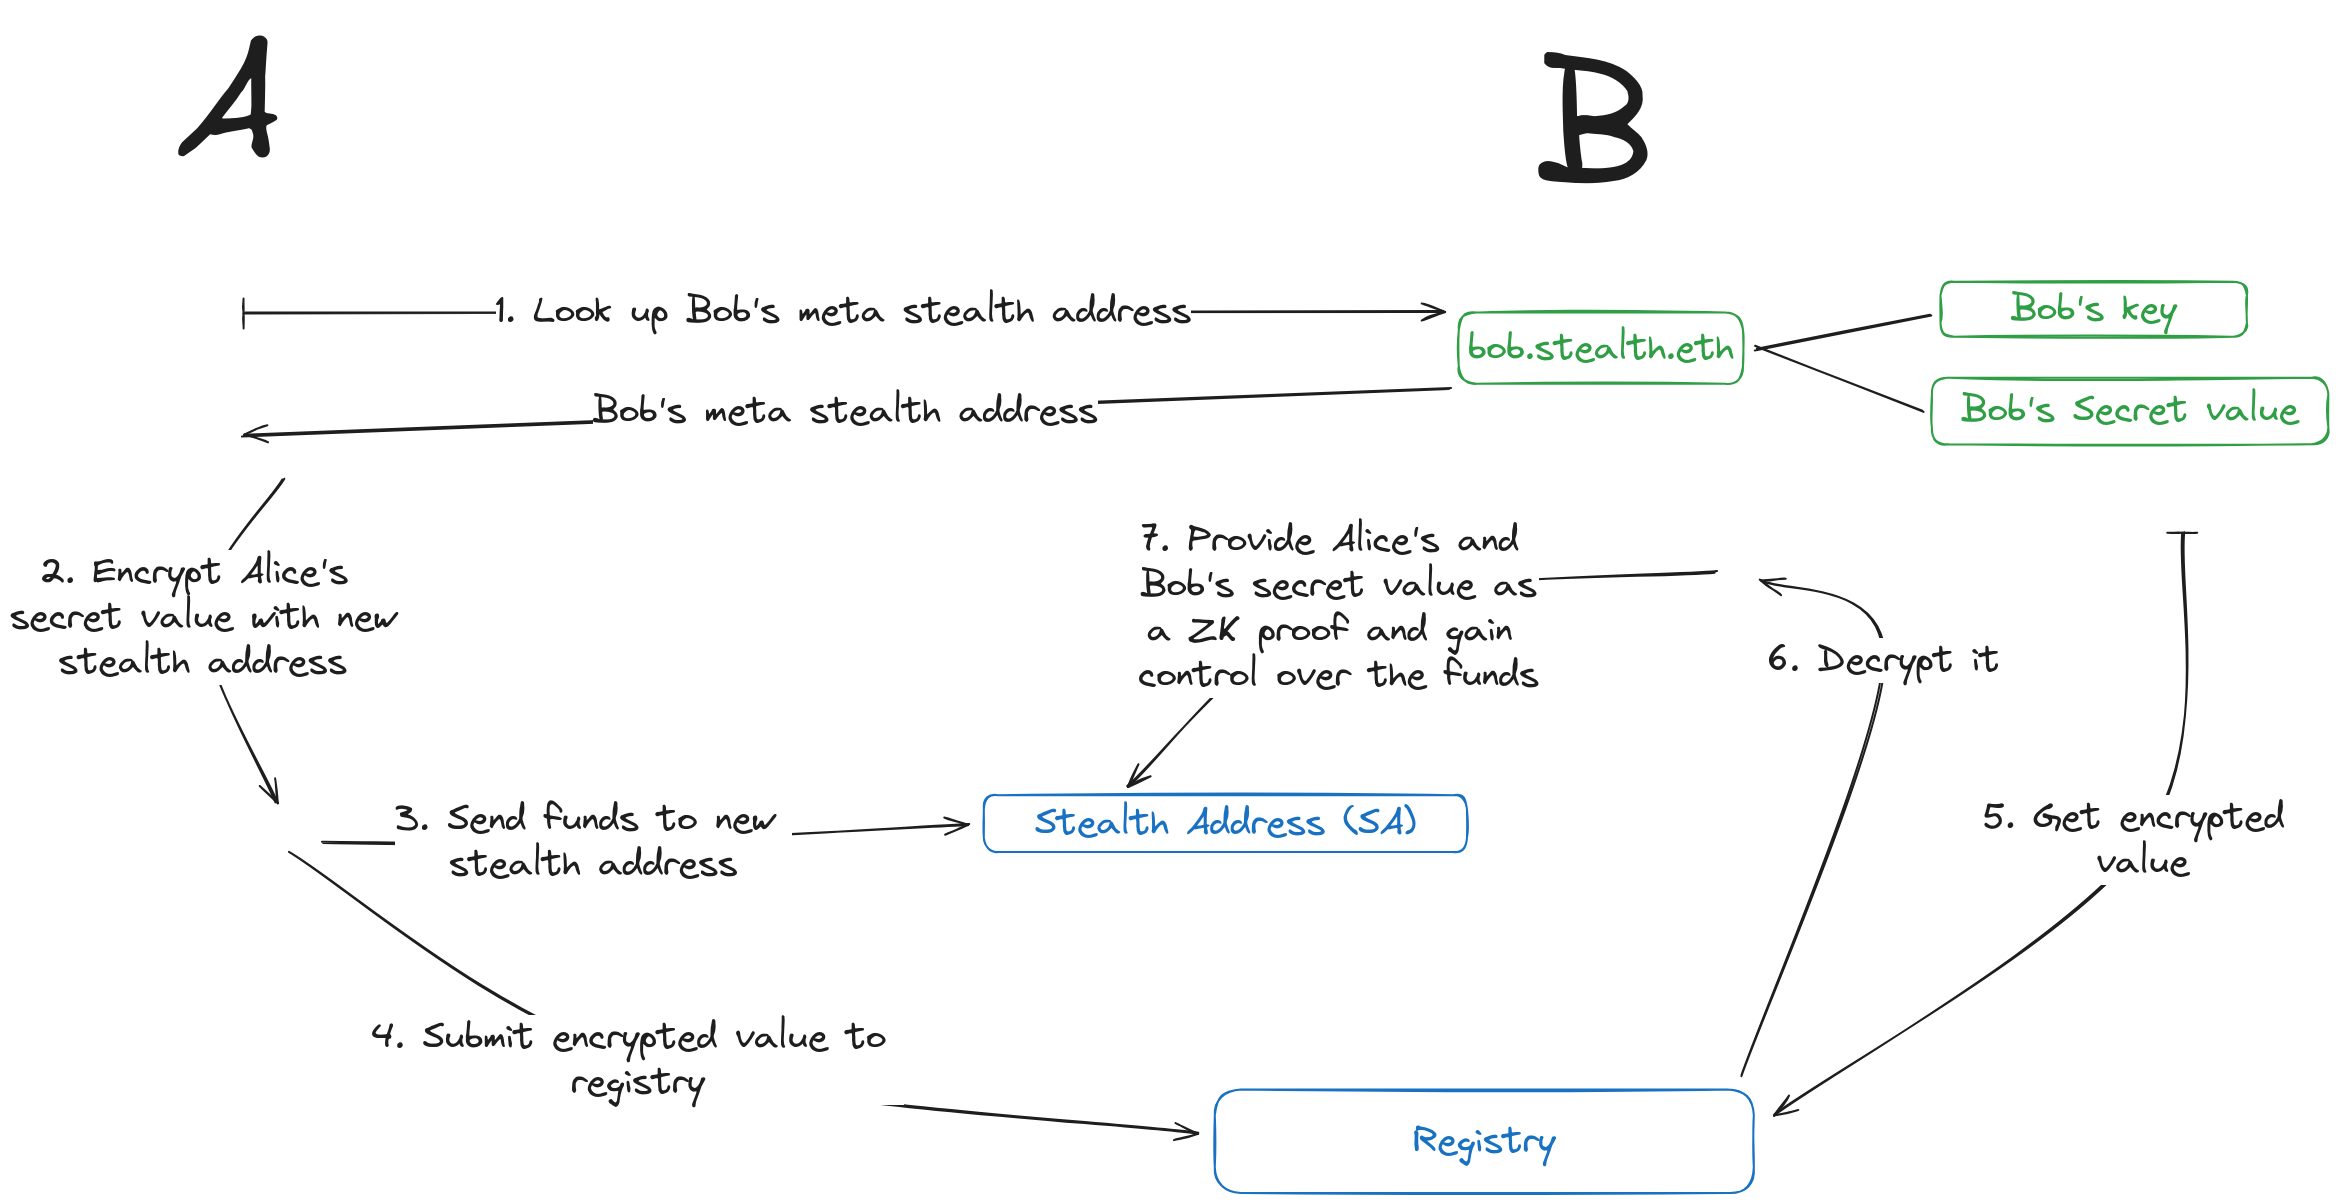
\includegraphics[scale=0.20]{assets/images/high-level.png}
    \caption{High Level Overview}
    \label{fig:hig-level}
	\cite{ButerinIncompleteGuide}
    \vspace{0.5cm}
\end{figure}

\section{Initial Setup}

Before Alice can send funds to Bob, Bob must first publish his meta stealth
address to some public location. Bob computes the following:

\begin{itemize}
	\item A private key $k$,
	\item A corresponding public key $K$,
	\item A secret value $x$,
	\item A hash of the secret value $h = hash(x)$.
\end{itemize}

Bob then publishes his meta stealth address in the form of a tuple $(K, h)$.
The hash is later used to prove to a stealth address contract that Bob is the
owner of the address and can spend funds sent to it.

\begin{figure}[h]
    \centering
    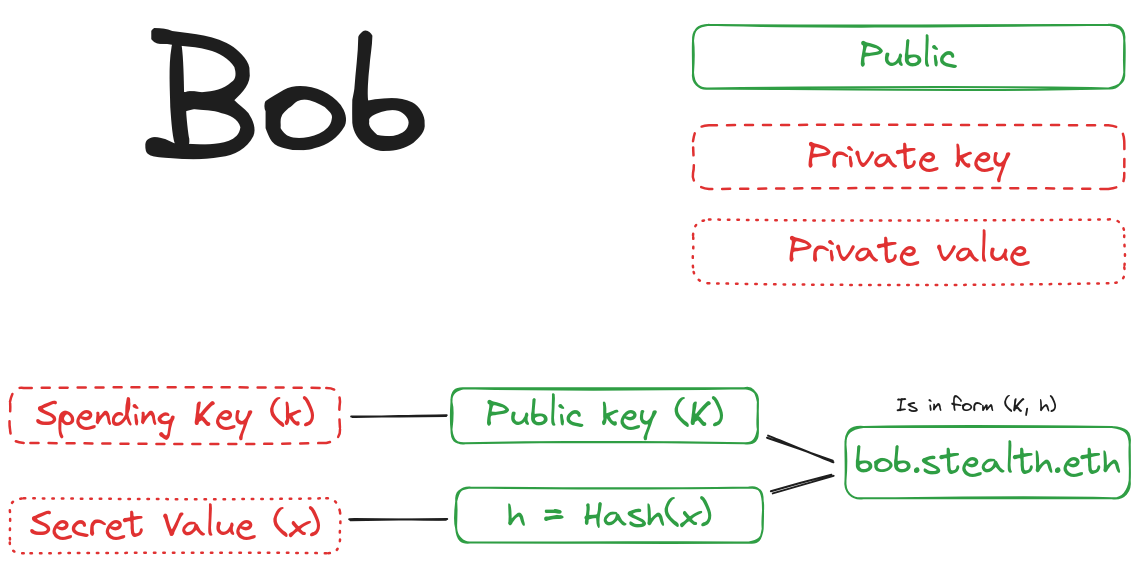
\includegraphics[scale=0.30]{assets/images/initial-setup.png}
    \caption{Initial Setup}
    \label{fig:initial-setup}
	\cite{ButerinIncompleteGuide}
    \vspace{0.5cm}
\end{figure}

\section{Sending Funds}

When Alice wishes to send funds to Bob, she must first generate a new stealth
address. Alice looks up Bob's meta stealth address $(K, h)$ and computes the
following:

\begin{itemize}
	\item A secret value $c$,
	\item A new random stealth address $SA$,
	\item An ephemeral key $P = encrypt(value=[c, SA], key=K)$,
	\item A code $C = hash(h, c)$.
\end{itemize}

Alice then creates a smart contract at the new stealth address $SA$, which contains
the code $C$ and sends funds to it. Then in the same transaction, Alice sends
the ephemeral key $P$ to public registry contract, which stores the ephemeral
keys for all stealth addresses.

\begin{figure}[h]
    \centering
    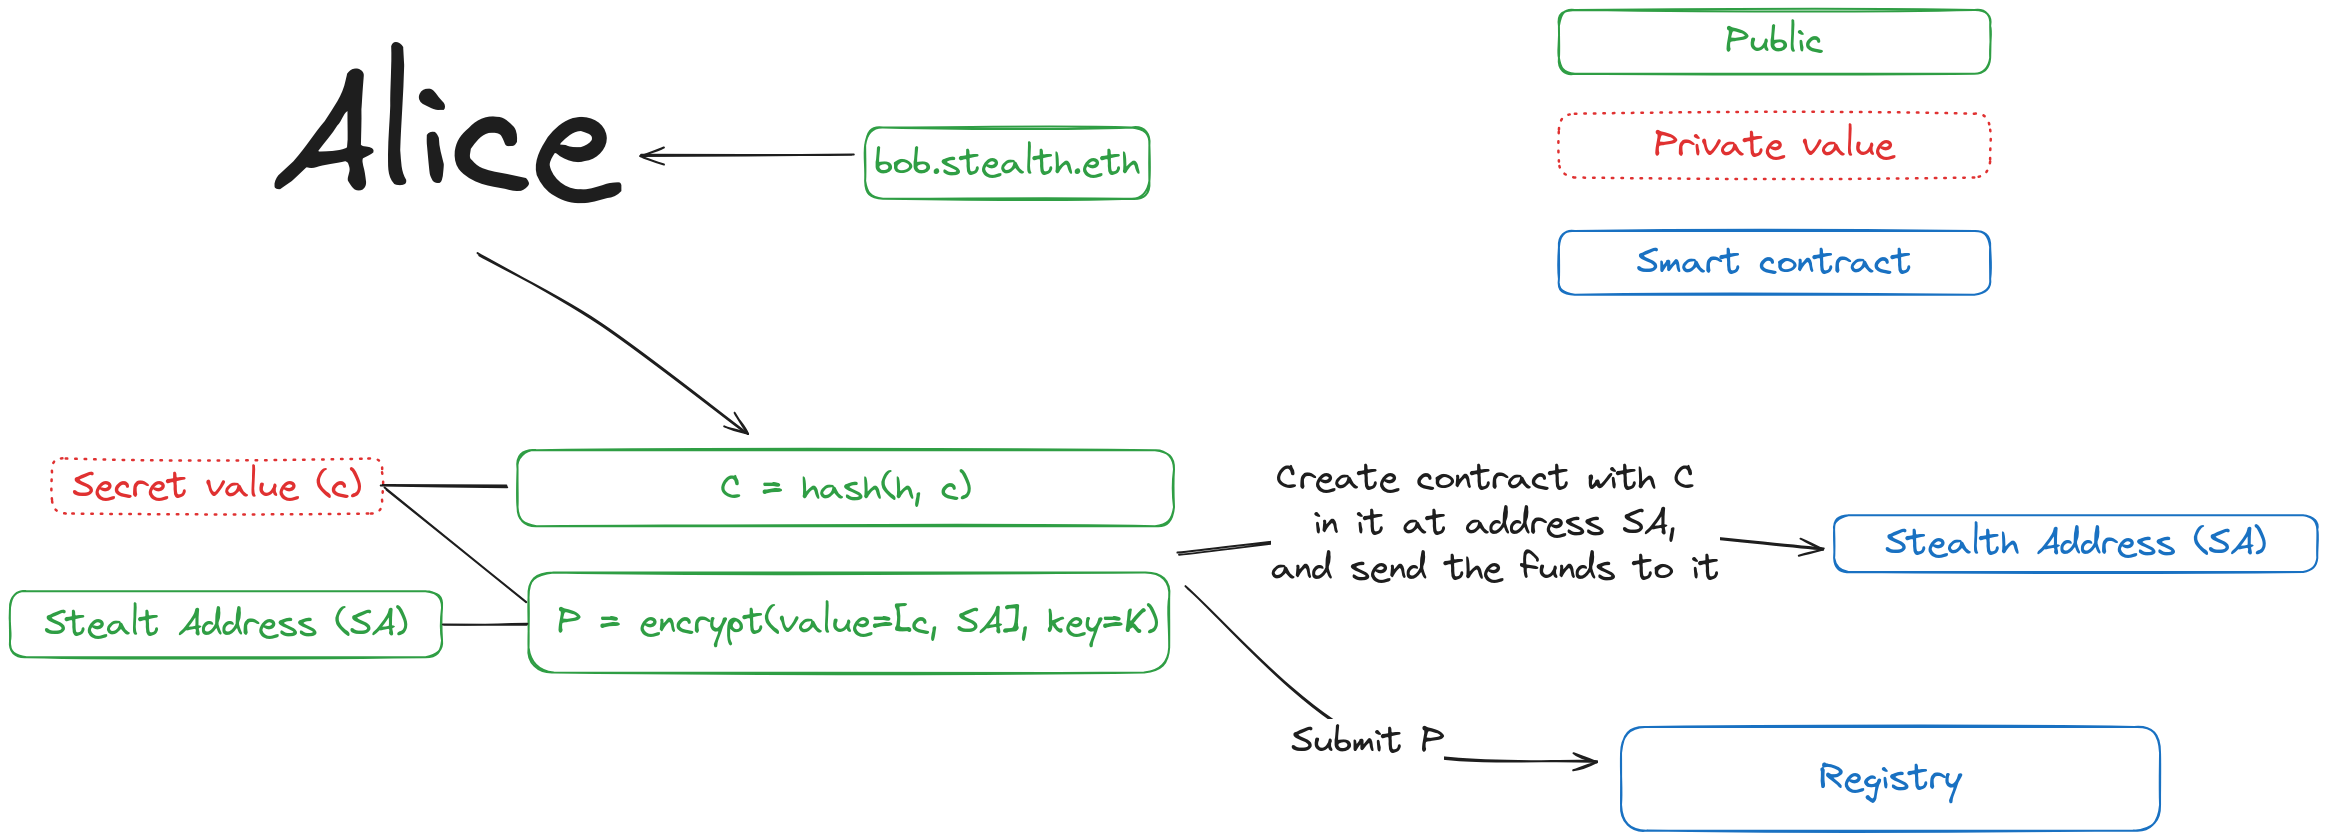
\includegraphics[scale=0.20]{assets/images/sending-funds.png}
    \caption{Sending Funds}
    \label{fig:sending-funds}
	\cite{ButerinIncompleteGuide}
    \vspace{0.5cm}
\end{figure}

\section{Scanning for Stealth Addresses}

Bob scans for stealth addresses by querying the public registry contract
from tha last point he scanned. The registry contract returns a list of
ephemeral keys. Bob then decrypts each ephemeral key with his private key $k$.
If the ephemeral key is meant for Bob, then it will contain the secret value
$c$ and the stealth address $SA$.

\section{Gaining control of Stealth Addresses}

Bob can gain control of the stealth address $SA$ by proving to the stealth
address contract that he is the owner of the values $x$ and $c$, such that\\
$C = hash(h, c) = hash(hash(x), c)$. Bob does this by computing a ZKP for 
this statement and sending it in a transaction from any address (preferably
not from any Bob's publicly known addresses) to the stealth address $SA$. The
$SA$ contract verifies the proof and if it isn't valid, the transaction is
rejected.

\section{Overview}

The whole solution design is illustrated in Figure \ref{fig:solution},
and was inspired by the work of Vitalik Buterin\cite{ButerinIncompleteGuide}.

\begin{figure}[h]
    \centering
    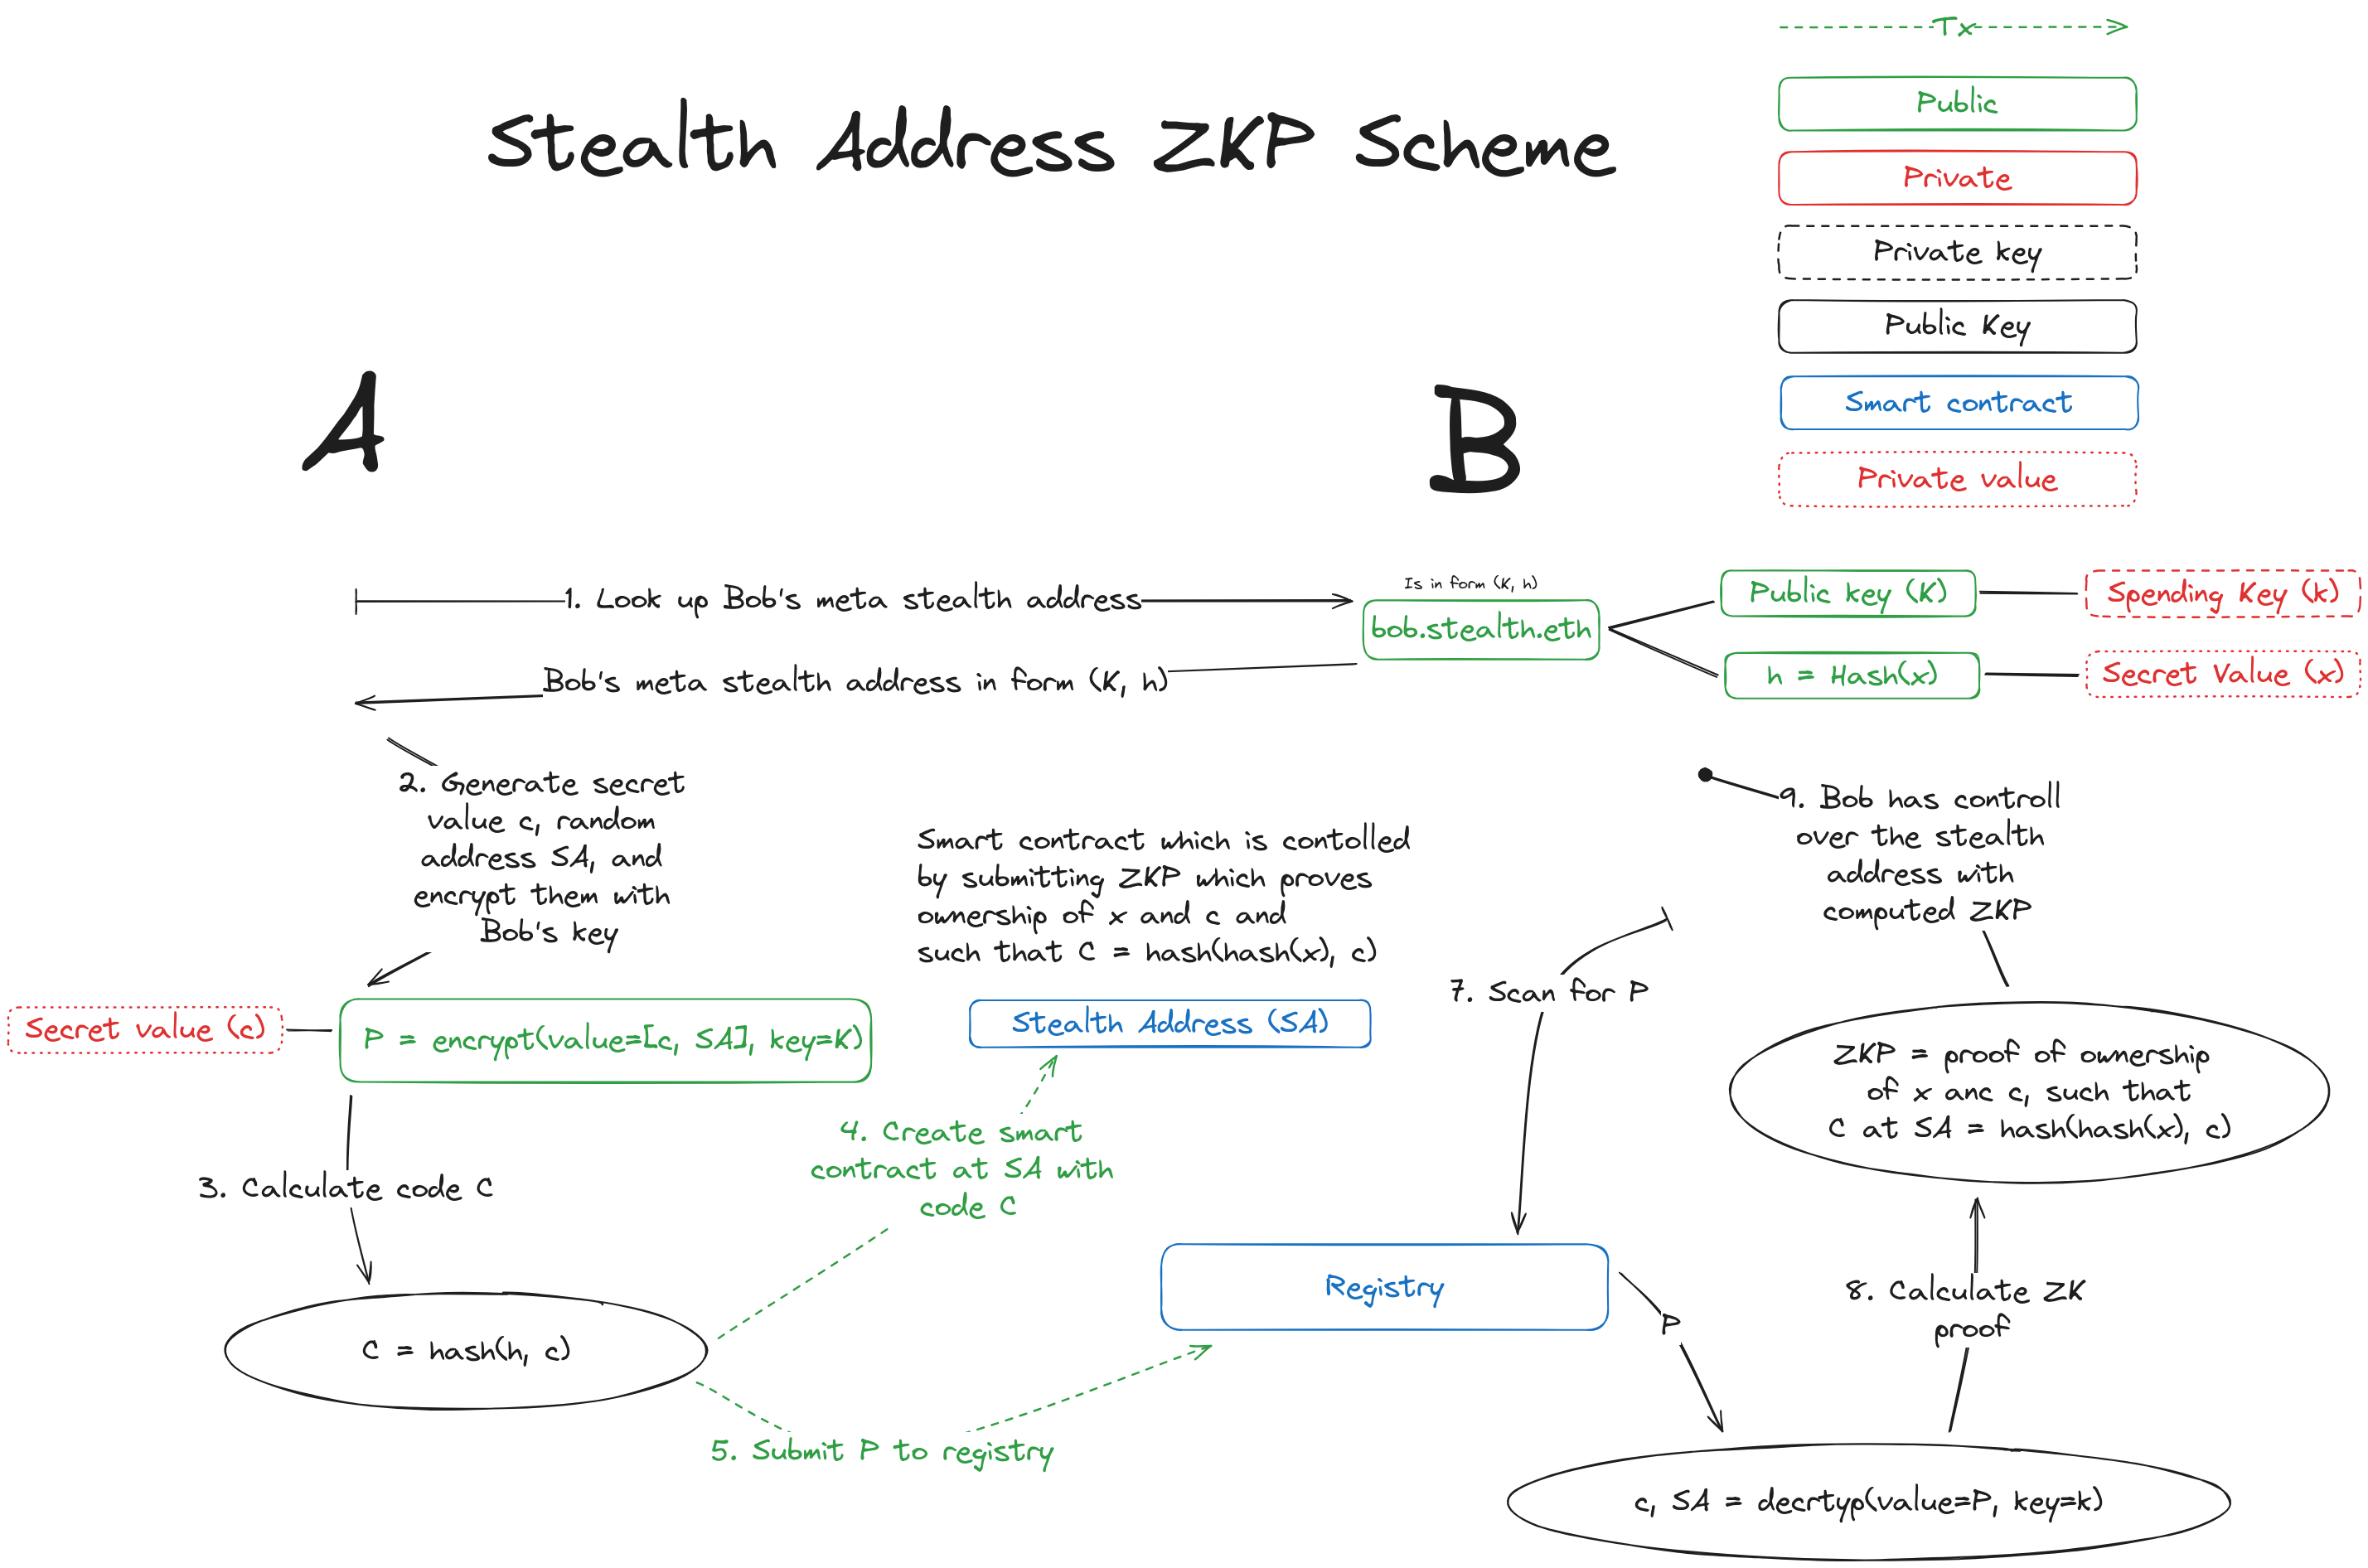
\includegraphics[scale=0.15]{assets/images/solution.png}
    \caption{Solution Design}
	\cite{ButerinIncompleteGuide}
    \label{fig:solution}
    \vspace{0.5cm}
\end{figure}

